\setchapterpreamble[u]{\margintoc}
\chapter{Electronic Mail Security}
\labch{chapter8}


Tipi di protocolli usati per trasferire mail:
\begin{itemize}
    \item Per spostare i messaggi tramite Internet dalla sorgente alla destinazione: Simple Mail Transfer Protocol (SMTP);
	\item Per trasferire messaggi tra server di posta: IMAP e POP sono i più comunemente usati.
\end{itemize}

SMTP:
\begin{itemize}
    \item Protocollo client-server basato su testo;
	\item Incapsula un messaggio di posta elettronica in una busta e inoltra i messaggi incapsulati dall'origine alla destinazione tramite più MTA;
	\item Viene spesso utilizzato il termine Extended SMTP (ESMTP) per riferirsi alle versioni successive di SMTP (2008).
\end{itemize}

Protocolli di accesso alla posta:
\begin{itemize}
    \item POP3 (Post Office Protocol): 
	\begin{itemize}
	    \item Consente a un client di posta elettronica di scaricare un'email da un server di posta (MTA);
		\item Gli user agent si connettono via TCP alla porta 110 del server;
		\item \item Dopo l'autorizzazione, l'UA può usare i comandi POP3 per recuperare ed eliminare la posta.
	\end{itemize}
	\item IMAP (Internet Mail Access Protocol):
	\begin{itemize}
	    \item Consente a un client di posta elettronica di accedere alla posta su un server email;
		\item Usa TCP sulla porta 143;
		\item È più complesso di POP3;
		\item Fornisce un'autenticazione più forte e funzioni non supportate da POP3.
	\end{itemize}
\end{itemize}

\subsection{RFC 5322}

Definisce un formato per i messaggi di testo inviati utilizzando email. I messaggi sono visti come una busta più un contenuto:
\begin{itemize}
    \item La busta contiene tutte le informazioni necessarie per effettuare la trasmissione e la consegna;
	\item Il contenuto compone l'oggetto da consegnare al destinatario;
	\item Lo standard RFC 5322 si applica solo ai contenuti;
	\item Lo standard del contenuto include una serie di campi di intestazione che possono essere utilizzati dal sistema di posta per creare la busta.
\end{itemize}

Lo schema SMTP/5322 ha pensanti limiti:
\begin{itemize}
    \item SMTP non può trasmettere file eseguibili o altri oggetti binari;
	\item SMTP non può trasmettere dati di testo che includono caratteri della lingua nazionale;
	\item I server SMTP possono rifiutare i messaggi di posta di una certa dimensione;
	\item I gateway SMTP che si occupano della traduzione da ASCII al codice carattere EBCDIC non utilizzano un insieme coerente di mappature, con conseguenti problemi di traduzione;
	\item Alcune implementazioni SMTP non aderiscono completamente agli standard.
\end{itemize}


\subsection{Multipurpose Internet Mail Extension (MIME)}

Estensione al framework RFC 5322 che ha lo scopo di affrontare alcuni dei problemi e delle limitazioni di SMTP. La specifica MIME include i seguenti elementi:
\begin{itemize}
    \item Vengono definiti cinque nuovi campi di intestazione del messaggio, che possono essere inclusi in un Intestazione RFC 5322. Questi campi forniscono informazioni sul corpo del messaggio;
	\item Vengono definiti diversi formati di contenuto, standardizzando così le rappresentazioni che supportano la posta elettronica multimediale;
	\item Sono definite codifiche di trasferimento che consentono la conversione di qualsiasi formato di contenuto in un modulo protetto da alterazioni al sistema di posta.
\end{itemize}

I cinque campi di intestazione definiti in MIME sono:
\begin{itemize}
    \item Versione MIME: Deve avere valore 1.0, per indicare che il messaggio è conforme a RFC 2045 e 2046;
	\item Tipo di contenuto: descrive i dati contenuti nel corpo con dettagli sufficienti affinché l'agent user ricevente possa scegliere un agente o un meccanismo appropriato per rappresentare i dati per l'utente o altrimenti trattare i dati in modo appropriato;
	\item Codifica di trasferimento dei dati: indica il tipo di trasformazione che è stata utilizzata per rappresentare il corpo del messaggio in un modo accettabile per il trasporto della posta;
	\item Content ID: Utilizzato per identificare le entità MIME in modo univoco in più contesti;
	\item Descrizione del contenuto: descrizione testuale dell'oggetto con il corpo (questo è utile quando l'oggetto non è leggibile).
\end{itemize}

Codifiche dei dati:
\begin{itemize}
    \item 7 bit: i dati sono tutti rappresentati da brevi righe di caratteri ASCII;
    \item 8 bit: le righe sono brevi, ma potrebbero essere presenti caratteri non ASCII;
    \item Binario: non solo possono essere presenti caratteri non ASCII, ma le righe non sono necessariamente sufficientemente corte per il trasporto SMTP;
    \item Quoted-printable: utile quando i dati sono costituiti da testo ASCII, la codifica è ampiamente riconoscibile dagli esseri umani;
    \item Base64: comunemente usato per codificare dati binari arbitrari in modo che non vengano modificati dal programma di mail-transport;
    \item x-token: codifica non standard
\end{itemize}

Nei primi tre casi non viene effettuata alcuna codifica. Il campo in questo caso serve solo per specificare info sulla natura del dato.

Un concetto importante in MIME e S/MIME è quello di forma canonica. La forma canonica è un formato, appropriato al tipo di contenuto, standardizzato per l'uso tra i sistemi. Ciò è in contrasto con la forma nativa, che è un formato che può essere peculiare di un particolare sistema.

\section{Email security}

Le mail sono soggette a più minacce:
\begin{itemize}
    \item Minacce relative all'autenticità: accesso non autorizzato al sistema di posta elettronica di un'azienda;
	\item Minacce legate all'integrità: modifica non autorizzata del contenuto dell'e-mail;
	\item Minacce legate alla riservatezza: divulgazione non autorizzata di informazioni sensibili;
	\item Minacce relative alla disponibilità: impedimento agli utenti finali di inviare o ricevere posta.
\end{itemize}

Protocolli contro le minacce

I protocolli standardizzati per contrastare le minacce sono:
\begin{itemize}
    \item STARTTLS: estensione di sicurezza di SMPT che fornisce autenticazione, integrità, non ripudiabilità e riservatezza per l'intero messaggio SMTP eseguendo SMTP su TLS;
	\item S/MIME: fornisce autenticazione, integrità, non ripudiabilità e riservatezza del corpo del messaggio trasportato in messaggi SMTP;
	\item DNSSEC (DNS security extention): fornisce autenticazione e protezione dell'integrità dei dati DNS ed è uno strumento utilizzato da vari protocolli di sicurezza della posta elettronica;
	\item DAME (DNS-based Authentication of Named Entities): progettato per superare problemi nel sistema delle CA fornendo un canale alternativo per l'autenticazione delle chiavi pubbliche basate su DNSSEC, con il risultato che le stesse relazioni di fiducia utilizzate per certificare gli indirizzi IP vengono utilizzate per certificare i server che operano su tali indirizzi.
\end{itemize}

\subsection{S/MIME}

Miglioramento della sicurezza dello standard MIME basato sulla tecnologia di RSA Data Security.
I servizi che offre sono:
\begin{itemize}
    \item Firma digitale con RSA/SHA-256;
	\item Cifratura dei messaggi con AES-128 con block chain;
	\item Compressione;
	\item Compatibilità email.
\end{itemize}

Autenticazione: fornita tramite firma digitale. Passi:
\begin{itemize}
    \item Il mittente crea il messaggio;
	\item Viene usato SHA-256 (one-way function) per creare un messaggio digest di 256 bit;
	\item Il digest viene cifrato con RSA utilizzando la chiave privata del mittente e il risultato viene aggiunto al messaggio. Vengono inoltre aggiunte le informazioni di identificazione per il firmatario, che consentiranno al destinatario di recuperare la chiave pubblica del firmatario;
	\item Il destinatario utilizza RSA con la chiave pubblica del mittente per decrittografare e recuperare il digest del messaggio;
	\item Il destinatario calcola il digest del messaggio per il messaggio e lo confronta con il codice hash decrittografato. Se i due corrispondono, il messaggio viene accettato come autentico.
\end{itemize}

Vengono accettate anche firme inviate separate dal messaggio che firmano. Queste possono essere usate per effettuare controlli successivi sul messaggio (es: rilevare successivamente se il programma è stato infettato da virus).

Confidenzialità: garantita cifrando i messaggi con AES con una chiave a 128 bit, con la modalità Cipher Block Chaining (CBC). Anche la chiave stessa è crittografata, in genere con RSA (quindi meccanismo chiave pubblica). Ciascuna chiave simmetrica viene utilizzata una sola volta:
\begin{itemize}
    \item Viene generata una nuova chiave come numero casuale per ciascun messaggio;
	\item Poiché deve essere utilizzata una sola volta, la chiave è vincolata al messaggio e trasmessa con esso;
	\item Per ridurre i tempi di crittografia, viene utilizzata la combinazione di crittografia simmetrica (per il contenuto del messaggio) e a chiave pubblica (per la chiave);
	\item Solo il destinatario è in grado di recuperare la chiave contenuta nel messaggio, in quanto è necessaria la sua chiave private per decifrarla.
\end{itemize}
	
Compatibilità mail: molti sistemi di posta elettronica consentono solo l'uso di blocchi che contengono testo ASCII. Per soddisfare questa restrizione, S/MIME fornisce il servizio di conversione.

Compressione: la compressione, opzionale, permette di risparmiare spazio sia per la trasmissione di mail che per lo storage dei file. La compressione può essere applicata in qualsiasi ordine rispetto alle operazioni di firma e crittografia dei messaggi. 

S/MIME usa i seguenti content type:
\begin{itemize}
    \item Dati (questo si riferisce ai tipi di contenuto del messaggio di MIME): si riferisce al contenuto gestito da MIME, che potrebbe poi essere incapsulato in un tipo SignedData, EnvelopedData o CompressedData;
	\item SignedData: usato per applicare la firma digitale al messaggio, contiene le info relative alla firma. Passi:
	\begin{itemize}
	    \item Seleziono un algoritmo di digest del messaggio (SHA o MD5 -> MD5 è sconsigliato);
		\item Calcolo il message digest (funzione hash) del contenuto da firmare;
		\item Cifro il digest con la chiave privata del firmatario;
		\item Preparo un blocco con le info per calcolare e confrontare il digest.
	\end{itemize}
	\item EnvelopedData: contiene i dati cifrati e le chiavi di cifratura. Passi:
	\begin{itemize}
	    \item Genero la chiave di sessioni con funzione pseudorandom per l'algoritmo di cifratura;
		\item Cifro la chiave di sessione con la chiave pubblica del destinatario;
		\item Preparo un blocco con le info necessarie al destinatario per decifrare;
		\item Cifro il messaggio.
	\end{itemize}
	\item CompressedData: usato per applicare compressione al messaggio.
\end{itemize}

Sicurezza di un'entità MIME:
\begin{itemize}
    \item S/MIME protegge un'entità MIME con una firma, una crittografia o entrambe;
	\item All'entità protetta vengono poi aggiunte una serie di info relative alla sicurezza, come certificati e ID degli algoritmi usati;
	\item Il tutto viene processato in un oggetto PKCS, che viene considerato come il contenuto del messaggio e wrappato in MIME.
\end{itemize}

Gestione dei certificati in S/MIME:
\begin{itemize}
    \item S/MIME utilizza certificati conformi alla versione 3 di X.509;
	\item I gestori e/o gli utenti S/MIME devono configurare ogni client con un elenco di chiavi attendibili e con elenchi di revoche di certificati. La responsabilità è locale per il mantenimento dei certificati necessari per verificare le firme in entrata e per crittografare i messaggi in uscita;
\end{itemize}

Gli user-agent di S/MIME svolgono una serie di funzioni legate alle chiavi:
\begin{itemize}
    \item Generazione delle chiavi;
	\item Registrazione: La chiave pubblica di un utente deve essere registrata con una autorità di certificazione per ricevere un certificato di chiave pubblica X.509;
	\item Archivio e recupero dei certificati.
\end{itemize}

RFC 2634 definisce una serie di servizi di sicurezza migliorati per S/MIME:
\begin{itemize}
    \item Signed receipt: la restituzione di una ricevuta firmata fornisce la prova della consegna al mittente del messaggio e gli consente di dimostrare a una terza parte che il destinatario ha ricevuto il messaggio;
	\item Security labels: insieme di informazioni di sicurezza relative alla sensibilità del contenuto protetto dall'incapsulamento S/MIME. Può essere utilizzato per il controllo degli accessi o determinarne la priorità;
	\item Secure mailing lists: ricevo un singolo messaggi, eseguire la crittografia specifica per ciascun membro della lista e lo inoltro a ogni destinatario;
	\item Signing certificates: questo servizio viene utilizzato per vincolare in modo sicuro il certificato del mittente alla propria firma tramite un attributo specifico.
\end{itemize}

\subsection{DNSSEC}

DNS (Domain Name System) è un servizio di ricerca che fornisce una mappatura tra il nome di un host su Internet e il suo indirizzo IP. Si compone di quattro elementi:
\begin{itemize}
    \item Domain Name Space: uno spazio dei nomi con struttura ad albero per identificare le risorse della rete;
	\item Database DNS: DB gerarchico costituito da record di risorse (RR) contenenti nomi, indirizzi IP, …;
	\item Name server: server che contengono informazioni su DNS e RR;
	\item Risolutori: programmi che estraggono informazioni dai name server per risolvere le richieste dei client.
\end{itemize}

Il DNS si basa su un database gerarchico contenente record di risorse (RR) che includono il nome, l'indirizzo IP e altre informazioni sugli host. Le caratteristiche principali del DATABASE DNS sono:
\begin{itemize}
    \item Gerarchia a profondità variabile per i nomi: consente un livello illimitato separato da ".";
	\item Database distribuito: esistono più server DNS sparsi in Internet;
	\item Distribuzione controllata dal database: il database è suddiviso in molteplici zone.
\end{itemize}

Esempio di risoluzione di un nome:
\begin{enumerate}
    \item Il programma utente richiede l'indirizzo IP per il nome del server;
	\item Il risolutore tenta di risolvere con i dati nella sua cache, altrimenti l'ISP interroga un server dei nomi locale;
	\item L'ISP trova l'indirizzo IP nel suo database locale o interroga altri server dei nomi;
	\item Quando la risposta viene ricevuta nel locale name server è memorizzato nella cache;
	\item Il programma utente riceve un indirizzo IP o un messaggio di errore.
\end{enumerate}

DNSSEC: 
\begin{itemize}
    \item Estensione con sicurezza di DNS;
	\item Fornisce protezione end-to-end tramite l'uso di firme digitali create dagli amministratori di zona e verificate dal software di risoluzione del destinatario;
	\item Evita la necessità di considerare attendibili server dei nomi e risolutori intermedi. Si crea infatti una catena di trust tra gli zone administrator, ciascuno dei quali garantisce per la propria zona;
	\item Consiste in un insieme di nuovi tipi di record di risorse e modifiche al protocollo DNS esistente;
\end{itemize}
	
In sostanza, DNSSEC è progettato per proteggere i client DNS dall'accettazione di record di risorse DNS contraffatti o alterati. Lo fa utilizzando le firme digitali per fornire:
\begin{itemize}
    \item Autenticazione dell'origine dei dati: garantisce che i dati provengano dalla fonte corretta (amministratore della zona DNS);
	\item Verifica dell'integrità dei dati: garantisce che il contenuto di un record di risorse (RR) non sia stato modificato.
\end{itemize}

La fiducia nella chiave pubblica della sorgente (dell'amministratore della zona DNS) è stabilita partendo da una zona di fiducia e stabilendo la catena di fiducia fino all'attuale fonte di risposta attraverso successive verifiche di firma della chiave pubblica di un figlio da parte del suo genitore. La chiave pubblica di una zona trusted è chiamata anchor trust.

DNSSEC aggiunge una serie di nuovi campi ai record di risorse (RR), per info sulle firme o per dire che quel name server non è parte di una determinata zona fornendo la lista di nomi del DNS (NSEC).
DNSSEC si basa sullo stabilire l'autenticità della gerarchia NDS che porta al domain name che mi interessa, e quindi dipende dalla root da cui inizio. La catena di autenticazione che va dalla mia root fino al domain name viene creata tramite autenticazione tra zone DNS. Per proteggere tutte le ricerche DNS, comprese quelle per nomi di dominio e tipi di record inesistenti, DNSSEC utilizza il record di risorse NSEC per autenticare le risposte negative alle query (serve per autenticare che la risposta "il domain name non esiste" arriva effettivamente dal server).

\subsection{DANE}

Protocollo che consente ai certificati X.509, comunemente usati in TLS, di essere associati ai nomi DNS tramite DNSSEC. Viene proposto come un modo per autenticare client e server TLS senza una CA. Lo scopo di DANE è sostituire l'affidarsi alla sicurezza del sistema delle CA con quello di DNSSEC.

DANE definisce un nuovo tipo di record DNS, TLSA, che può essere usato come metodo sicuro per autenticare certificati SSL/TLS. Questo record vincola l'emissione e la consegna del certificato a un dato dominio:
\begin{itemize}
    \item Il proprietario del dominio del server crea il record TLSA che identifica il certificato;
	\item Quando il client riceve il certificato, cerca il relativo record TLSA per quel dominio e confronta i dati del record con il certificato.
\end{itemize}

Poco diffuso.

\section{Sender Policy Framework (SPF)}

SPF è il metodo standardizzato per validare se il mittente della mail è autorizzato ad usare quello specifico dominio (permette di identificare mail forgiate, sta alla base del sistema di spam). 
Funzionamento:
\begin{itemize}
    \item Il proprietario di un dominio specifica la propria policy di invio della posta (es: quali server di posta utilizzano per inviare posta dal loro dominio);
	\item Il proprietario del dominio pubblica queste informazioni in un record SPF nella zona DNS del dominio;
	\item Quando il server di posta di qualcun altro riceve un messaggio che afferma di provenire da quel dominio, il server ricevente può verificare se il messaggio è conforme alla policy dichiarata del dominio (es: se il messaggio proviene da un server sconosciuto, può essere considerato un falso).
\end{itemize}

I record SPF vengono controllati nel momento in cui accedo al DNS.

\begin{figure}[h]
    \centering
    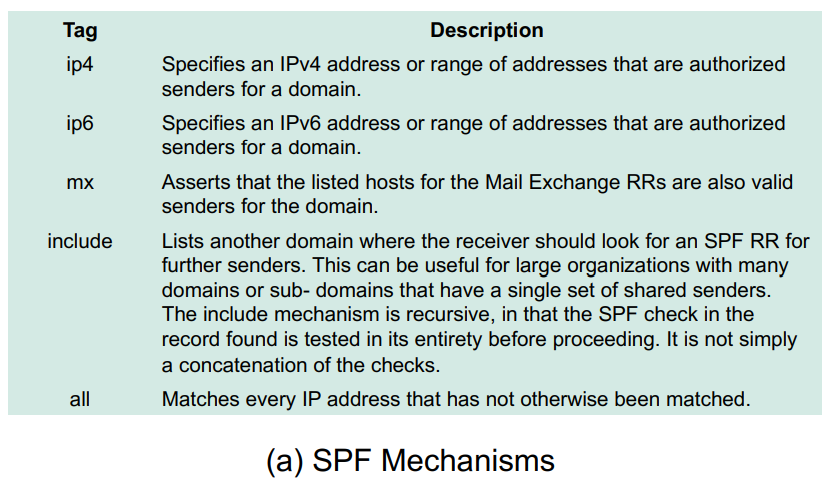
\includegraphics[width=1\textwidth]{images/chapter8/8-1.png}
    \caption{Reti wireless.}
    \label{fig:8-1}
\end{figure}

\begin{figure}[h]
    \centering
    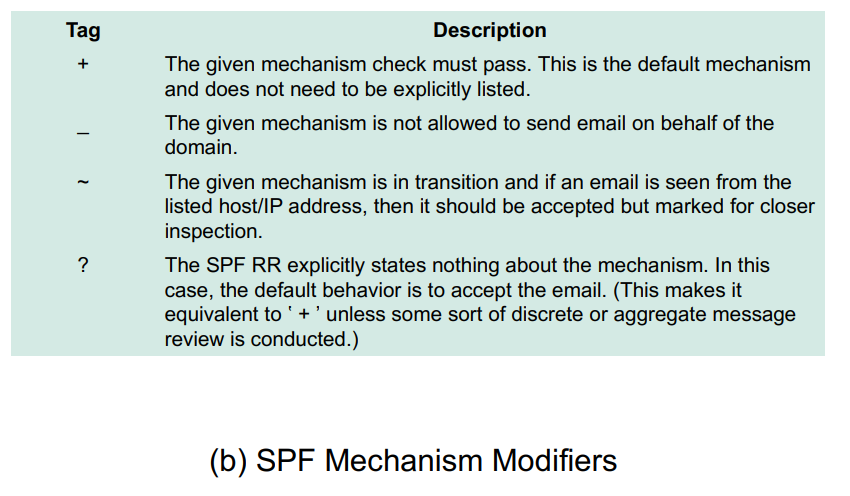
\includegraphics[width=1\textwidth]{images/chapter8/8-2.png}
    \caption{Reti wireless.}
    \label{fig:8-2}
\end{figure}

\section{DomainKeys Identified Mail (DKIM)}

Specifica per la firma crittografica dei messaggi di posta elettronica, che consente a un dominio di firma di rivendicare la responsabilità di un messaggio nel flusso di posta. Sostanzialmente permette ai responmsabili del dominio di garantire la validutà della mail (es: gmail garantisce la validità della mail). I destinatari del messaggio possono verificare la firma interrogando direttamente il dominio del firmatario per recuperare la chiave pubblica appropriata e possono così confermare che il messaggio è stato attestato da un soggetto in possesso della chiave privata del dominio di firma. È stato ampiamente adottato da una serie di provider di posta elettronica e ISP (gmail, yahoo, ecc.) .

Strategia:
\begin{itemize}
    \item DKIM fornisce una tecnica di autenticazione e-mail trasparente per l'utente finale;
	\item Il messaggio di posta elettronica di un utente è firmato da una chiave privata del dominio amministrativo da cui ha origine l'e-mail;
	\item La firma copre tutto il contenuto del messaggio e parte dell'header;
	\item Il ricevente può accedere alla chiave pubblica corrispondente tramite un DNS e verificare la firma, autenticando così che il messaggio provenga dal dominio amministrativo rivendicato. 
	\item Questo approccio è diverso da quello di S/MIME, che utilizza la chiave privata del mittente per firmare il contenuto del messaggio.
\end{itemize}

\section{Domain-Based Message Authentication, Reporting, and Conformance (DMARC)}

Consente ai mittenti di posta elettronica di specificare la politica su come gestire la posta, i tipi di rapporti che i destinatari possono inviare e la frequenza con cui tali rapporti dovrebbero essere inviati.

DMARC funziona con SPF e DKIM:
\begin{itemize}
    \item SPF e DKIM consentono ai mittenti di avvisare i destinatari, tramite DNS, se una mail del mittente è valida e se deve essere consegnata, contrassegnata o eliminata;
	\item Né SPF né DKIM includono un meccanismo per dire ai ricevitori se essi sono in uso, né dispongono di meccanismi di feedback per informare i mittenti dell'efficacia delle tecniche anti-spam;
\end{itemize}

DMARC risolve questi problemi essenzialmente standardizzando il modo in cui i ricevitori di posta elettronica eseguono l'autenticazione e-mail utilizzando i meccanismi SPF e DKIM

